\documentclass{article}
\usepackage{graphicx} % Required for inserting images

\title{Zadanie 2}
\author{Damian Rogalski}
\date{Maj 2024}

\begin{document}

\maketitle

\section{Model spalania lasu}
Program początkowo losowo generuje las na podstawie współczynnika prawdopodobieństwa wygenerowania drzewa. Następnie wywołana funkcja burnForest losowo wybiera startowy punkt rozpoczęcia pożaru. Jeżeli jest nim drzewo to program zaczyna wyszukiwać przyległych drzew (na górze, dole, obok i po ukosie). Jeżeli program znajdzie drzewo to je podpala. Gdy program nie może już znaleźć kolejnych drzew to zwraca spalony las. Jako dodatkowy parametr możemy uwzględnić wiatr w symulacji. Struktura wiatru posiada siłę oraz kierunek. Po zadaniu kierunku i siły wiatru wybór kolejnych drzew przesuwa się we wskazanym zwrocie po ilości drzew równej sile wiatru. Dalsza część działania programu odbywa się jak w bazowej wersji. 

\section{Wyniki symulacji}
Dla współczynnika prawdopodobieństwa wygenerowania drzewa rzędu 43\% i lasu wielkości 100x100 program zwraca wyniki spalenia powierzchni lasu rzędu 36\%. Ponadto program dla 10000 prób z losowym współczynnikiem wylicza optymalny współczynnik zalesienia, jednakże wyniki są niejednoznaczne i wahają się miedzy 2 a 40\%. Utrudnia to jednoznaczną analizę, jednakże najczęściej otrzymywałem wyniki około 13\%. Jeżeli do symulacji dodamy wpływ wiatru o sile 2 i kierunku w prawo procentowe wyniki spalenia całej powierzchni lasu wynoszą około między 9\% a 30\%, natomiast optymalny stopień zalesienia oscyluje wokół 2\%.

\newpage

\section{Graficzne przedstawienie wyników}
\subsection{Symulacja bez uwzględnienia wiatru}
\begin{figure}[h]
    \begin{minipage}{0.5\textwidth}
        \centering
        
\includegraphics[width=\linewidth]{original_forest.png}
        \caption{Wygenerowany las ze współczynnikiem zalesienia 43\%}
    \end{minipage}\hfill
    \hskip 1em
    \begin{minipage}{0.5\textwidth}
        \centering
        
        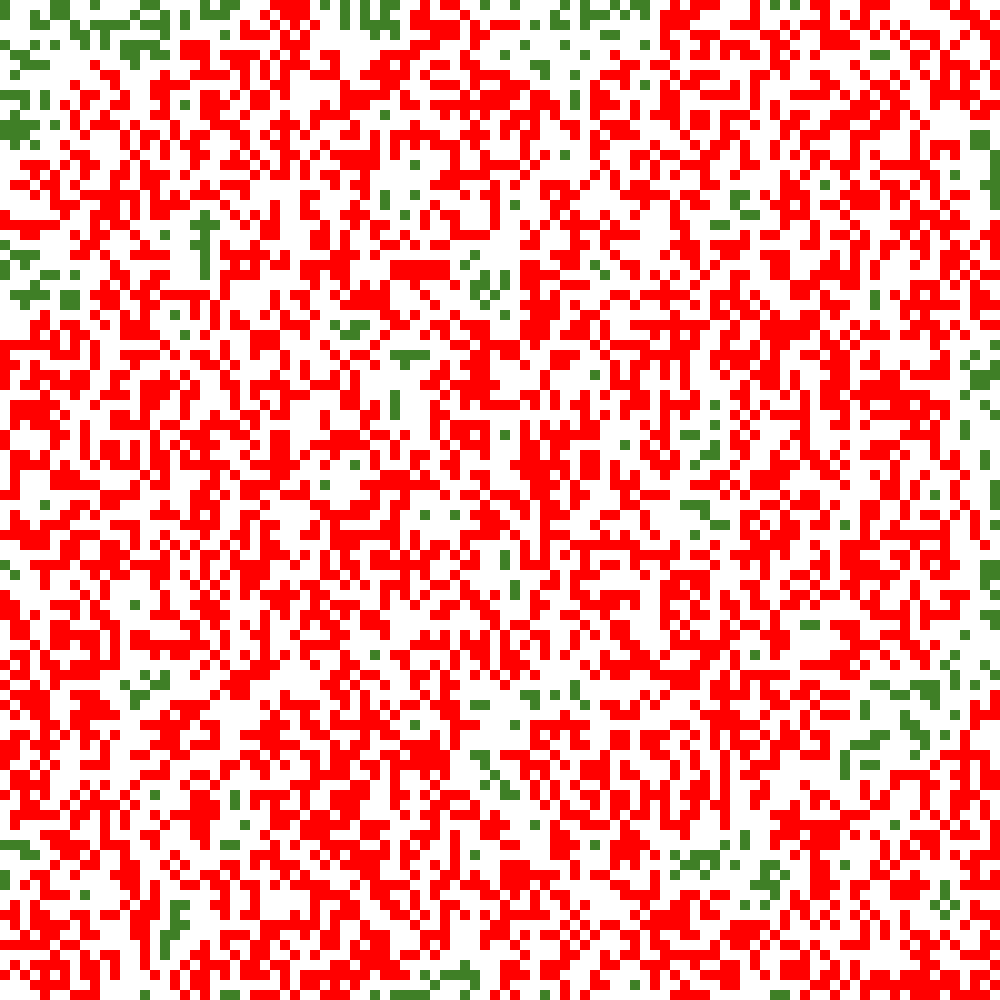
\includegraphics[width=\linewidth]{burnt_forest.png}
        \caption{Las po wykonaniu symulacji, procent spalenia to 36.8\%}
    \end{minipage}\hfill
    \hskip 1em
    \begin{minipage}{0.5\textwidth}
        \centering
        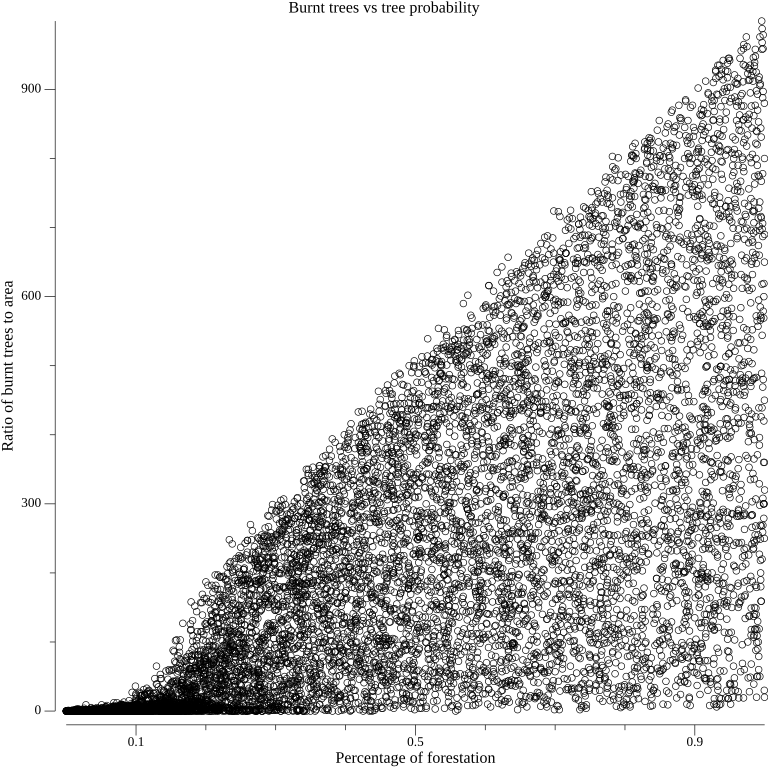
\includegraphics[width=\linewidth]{burnt_trees.png}
        \caption{Wykres stopnia zalesienia do spalonej powierzchni lasu}
    \end{minipage}
\end{figure}

\newpage

\subsection{Symulacja z uwzględnieniem wiatru (kierunek: w prawo, siła: 2)}
\begin{figure}[h]
    \begin{minipage}{0.5\textwidth}
        \centering
        
\includegraphics[width=\linewidth]{original_forest_wind.png}
        \caption{Wygenerowany las ze współczynnikiem zalesienia 43\%}
    \end{minipage}\hfill
    \hskip 1em
    \begin{minipage}{0.5\textwidth}
        \centering
        
        
\includegraphics[width=\linewidth]{burnt_forest_wind.png}
        \caption{Las po wykonaniu symulacji, procent spalenia to 29.39\%}
    \end{minipage}\hfill
    \hskip 1em
    \begin{minipage}{0.5\textwidth}
        \centering
        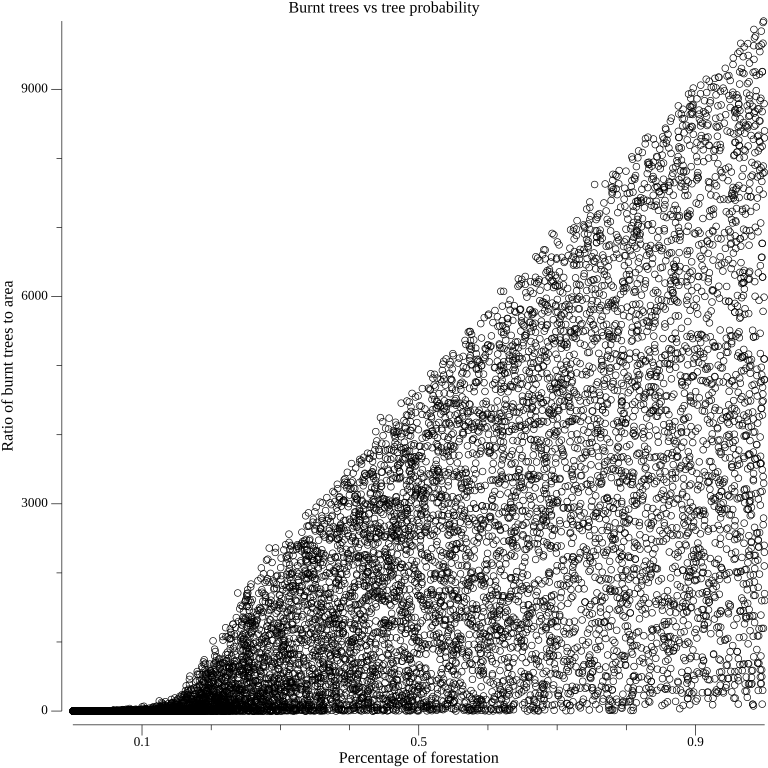
\includegraphics[width=\linewidth]{burnt_trees_wind.png}
        \caption{Wykres stopnia zalesienia do spalonej powierzchni lasu}
    \end{minipage}
\end{figure}

\end{document}
